% !TeX spellcheck = en_US

\chapter{Add new package manager module}\label{chap:add}
This chapter will show extensibility of framework by adding new package manager module for $aptitude$ package manager.\\
Section \ref{sec:aptitude} provides common information about the package manager.\\
In section \ref{sec:aptitude_imp} module is implemented and in section \ref{sec:aptitude_int} is integrated into bash language module

\section{Aptitude}\label{sec:aptitude}
This section describes the $aptitude$ package manager.
Like $apt$-$get$ is $aptitude$ command line program and just like the $apt$-$get$ a package can be installed using command $aptitude$ $install$ \emph{package}. In additional it can be started in pseudo-graphic mode, to provide visual interface (figure \ref{fig:aptitude_gui}).
\begin{figure}[ht]   
	\centering
	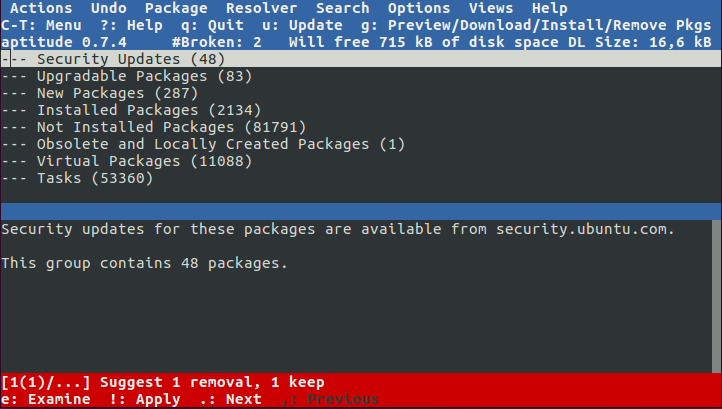
\includegraphics[width=0.7\textwidth]{Screenshot_aptitude.png}
	\caption{Command line visual interface for $aptitude$ package manager.}
	\label{fig:aptitude_gui}
\end{figure}
Another additional capability compared to $apt$-$get$ is a search for packages by a part of the name (or by other attributes) using the $aptitude$ $search$ command.
\section{Implementing new package manager module}\label{sec:aptitude_imp}
Process of the implementing of $aptitude$ will be described here.
At first $aptitude$ will be inherited from class $PackageManager$.
\begin{lstlisting}[caption={Aptitude inherited from PackageManager}\label{lst:aptit_inher},captionpos=t] 
public final class PM_aptitude extends PackageManager {
	@Override
	public void proceed(String filename, String source)
		throws FileNotFoundException, IOException, JAXBException {
		// TODO Auto-generated method stub
	}
	
}
\end{lstlisting}
Now common code is added, like constructor method and model's name.
\begin{lstlisting}[caption={Aptitude with common parametrs}\label{lst:aptit_common},captionpos=t] 
public final class PM_aptitude extends PackageManager {

	// package manager name
	static public final String Name = "aptitude";
	
	/**
	* Constructor
	*/
	public PM_aptitude(Language language, Control_references cr) {
		this.language = language;
		this.cr = cr;
	}
	
	@Override
	public void proceed(String filename, String source)
		throws FileNotFoundException, IOException, JAXBException {
		// TODO Auto-generated method stub
	}
}
\end{lstlisting}
Since package manager need to read files, the CSAR handler is stored cy constructor.
In addition the language is stored too, to be propagated later to Package Handler.\\
Now focus on $proceed$ function. Line-by-line analyzer is needed, which can modify the data and in this case file will be rewritten.

\begin{lstlisting}[caption={Aptitude proceed}\label{lst:aptit_proceed},captionpos=t]
	@Override
public void proceed(String filename, String source)
	throws FileNotFoundException, IOException, JAXBException {
	if (cr == null)
		throw new NullPointerException();
	System.out.println(Name + " proceed " + filename);
	BufferedReader br = new BufferedReader(new FileReader(filename));
	boolean isChanged = false;
	String line = null;
	String newFile = "";
	while ((line = br.readLine()) != null) {
		// TODO parsing will be done here
	}
	br.close();

	if (isChanged)
		Utils.createFile(filename,newFile);
}	 
\end{lstlisting}
$isChanged$ indicates when file must be rewritten with new content from $newFile$ variable.
Now an aptitude parser will be implemented, that reads one line from $line$ variable and stored it ore altered version to $newFile$.
Package installation calls will be detected, commented out and package name will be propagated to Package Handler.

\begin{lstlisting}[caption={Aptitude parse}\label{lst:aptit_parse},captionpos=t]
String[] words = line.replaceAll("[;&]", "").split("\\s+");
// skip space at the beginning of string
int i = 0;
if (words[i].equals(""))
	i = 1;
// look for apt-get
if (words.length >= 1 + i && words[i].equals("aptitude")) {
	// apt-get found
	if (words.length >= 3 + i && words[1 + i].equals("install")) {
		System.out.println("aptitude found:" + line);
		isChanged = true;
		for (int packet = 2 + i; packet < words.length; packet++) {
			System.out.println("packet: " + words[packet]);
			cr.getPacket(language, words[packet], source);
		}
	}
	newFile += "#//References resolver//" + line + '\n';
} else
	newFile += line + '\n';
\end{lstlisting}
For parsing purposes the line is divided into words. Packet Handler is called by $getPackage$ function.
\section{Integrating Aptitude into Bash module}\label{sec:aptitude_int}
Now the aptitude module will be added to Bash language.
The only one thing to do is a adding the $aptitude$ to Bash's set of package manager.
This is done during Bash's construction with a sting: \emph{"packetManagers.add(new PM\_aptitude(this, cr));"}.\\
Now the new package manager module is ready to work.